\section{Anforderungszuordnung}
\begin{figure}[htb]

	\centering

	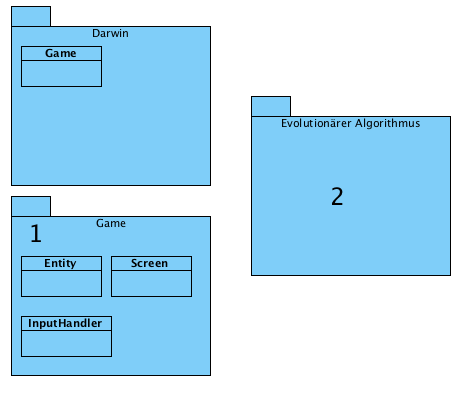
\includegraphics[width=7cm]{class.png}

	\caption{Momentane Package-Ansicht}

	\end{figure}
\begin{tabularx}{\textwidth}{|p{0.7cm}|p{7.0cm}|X|X|}
\hline
Nr. & Anforderung & 1 & 2 \\
\hline
1 & Spielbares Spiel & X & \\
\hline
2 & Lernfähige Gegner & X & X  \\
\hline
3 & Export-Funktion für Gegner & & X  \\
\hline
4 & Bot-Gegen-Bot-Modus & & X    \\
\hline
\end{tabularx}
